\documentclass[12pt]{article}
\usepackage[top=1in, bottom=1in, left=1in, right=1in]{geometry}
%\usepackage[margin=1in]{geometry}
\usepackage[onehalfspacing]{setspace}
%\usepackage[doublespacing]{setspace}
\usepackage{amsmath, amssymb, amsthm}
\usepackage{enumerate, enumitem}
\usepackage{fancyhdr, graphicx, proof, comment, multicol}
\usepackage[none]{hyphenat} % This command prevents hyphenation of words
\binoppenalty=\maxdimen % This command and the next prevent in-line equation breaks
\relpenalty=\maxdimen
%    Good website with common symbols
% http://www.artofproblemsolving.com/wiki/index.php/LaTeX%3ASymbols
%    How to change enumeration using enumitem package
% http://tex.stackexchange.com/questions/129951/enumerate-tag-using-the-alphabet-instead-of-numbers
%    Quick post on headers
% http://timmurphy.org/2010/08/07/headers-and-footers-in-latex-using-fancyhdr/
%    Info on alignat
% http://tex.stackexchange.com/questions/229799/align-words-next-to-the-numbering
% http://tex.stackexchange.com/questions/43102/how-to-subtract-two-equations
%    Text align left-center-right
% http://tex.stackexchange.com/questions/55472/how-to-make-text-aligned-left-center-right-in-the-same-line
\usepackage{microtype} % Modifies spacing between letters and words
\usepackage{mathpazo} % Modifies font. Optional package.
\usepackage{mdframed} % Required for boxed problems.
\usepackage{parskip} % Left justifies new paragraphs.
\linespread{1.1} 


%figure support
\usepackage{import}
\usepackage{xifthen}
\pdfminorversion=7
\usepackage{pdfpages}
\usepackage{transparent}
\newcommand{\incfig}[1]{%
	\def\svgwidth{\columnwidth}
	\import{./figures/}{#1.pdf_tex}
}
\graphicspath{ {./figures/} }
\pdfsuppresswarningpagegroup=1

\newenvironment{problem}[1]
{\begin{mdframed}[linewidth=0.8pt]
        \textsc{Problem #1:}

}
    {\end{mdframed}}

\newenvironment{solution}
    {\textsc{Solution:}\\}
    {\newpage}% puts a new page after the solution
    
\newenvironment{statement}[1]
{\begin{mdframed}[linewidth=0.6pt]
        \textsc{Statement #1:}

}
    {\end{mdframed}}

%\newenvironment{prf}
 %   {\textsc{Proof:}\\}
 %   {\newpage}% puts a new page after the solution

\begin{document}
% This is the Header
% Make sure you update this information!!!!
\noindent
\textbf{CIS4367.01} \hfill \textbf{Brandon Thompson} \\
\normalsize Prof. Elibol \hfill Due Date: 3/11/20 \\

% This is where you name your homework
\begin{center}
\textbf{Homework 10}
\end{center}
	\begin{problem}{\#5.1}
		Consider a simplified university database that includes information
		on courses (name, number, day, time, room number, max enrollment)
		and on faculty teaching courses and students attending courses.
		Suggest a relational database for efficiently managing this information.
	\end{problem}
	\begin{solution}
		Database is composed of 3 tables, Course table, Faculty table, Student table.
		The Student and Faculty tables are linked by the course number field in the Course table.
		\begin{center}
			\textbf{Course Table}\\
			\vspace{1em}
			\begin{tabular}{|c|c|c|c|c|c|}
				\hline
				\textbf{Course Name} & \textbf{Course Number} & \textbf{Day} & \textbf{Time} & \textbf{Room Number} & \textbf{Max Enrollment}\\
				\hline
				& Primary Key& & & &\\
				\hline
			\end{tabular}
		\end{center}
		\\
		\vspace{2.5em}
		\begin{center}
			\textbf{Student Table}\\
			\vspace{1em}
			\begin{tabular}{|c|c|}
				\hline
				\textbf{Student Name} & \textbf{Course Number}\\
				\hline
				& Foreign Key\\
				\hline
			\end{tabular}
		\end{center}
		\\
		\vspace{2.5em}
		\begin{center}
			\textbf{Faculty Table}\\
			\vspace{1em}
			\begin{tabular}{|c|c|}
				\hline
				\textbf{Faculty Name} & \textbf{Course Number}\\
				\hline 
				& Foreign Key\\
				\hline
			\end{tabular}
		\end{center}
	\end{solution}

	\begin{problem}{\#5.2}
		The following table below provides information on members of a mountain
		climbing club.
		\begin{center}
		\begin{tabular}{|c|c|c|c|}
			\hline
			\textbf{Climber-ID} & \textbf{Name} & \textbf{Skill Level} & \textbf{Age}\\
			\hline
			123 & Edmund & Experienced & 80\\
			\hline
			214 & Arnold & Beginner & 25\\
			\hline
			313 & Bridget & Experienced & 33\\
			\hline
			212 & James & Medium & 27\\
			\hline
		\end{tabular}
		\end{center}

		The primary key is \textit{Climber-ID}. Explain whether or not each of the
		following rows can be added to the table.
		\begin{center}
			\begin{tabular}{|c|c|c|c|}
				\hline				\textbf{Climber-ID} & \textbf{Name} & \textbf{Skill Level} & \textbf{Age}\\
				\hline
				214 & Abbot & Medium & 40\\
				\hline
				    & John & Experienced & 19\\
				\hline
				15 & Jeff & Medium & 42\\
				\hline
			\end{tabular}
		\end{center}
	\end{problem}
	\begin{solution}
		The first row in the second table cannot be added because there is already
		a row in the first table with that primary key. Primary keys need to be unique.

		The second row in the second table cannot be added because primary keys cannot
		be null or empty.

		The third row in the second table can be added because there is no other row
		that matches that primary key.
	\end{solution}

	\begin{problem}{\#5.4}
		We wish to create a student table containing the student's ID number, name,
		and telephone number. Write an SQL statement to accomplish this.
	\end{problem}
	\begin{solution}
		SQL statement to create tables within a database is:\\
		\\
		\verb|CREATE TABLE <table name> (|\\
		\verb|<column name> <data type>(<size>),|\\
		\verb|<column name> <data type>(<size>),|\\
		\verb|...|\\
		\verb|<column name> <data type>(<size>));|

		Command used to create student table:\\
		\\
		\verb|CREATE TABLE student (|\\
		\verb|student_ID INTEGER PRIMARY KEY,|\\
		\verb|firstName VARCHAR(20),|\\
		\verb|lastName VARCHAR(20),|\\
		\verb|phoneNumber CHAR(10));|\\
		\\
		Results in table:\\
		\begin{figure}[ht!]
			\centering
			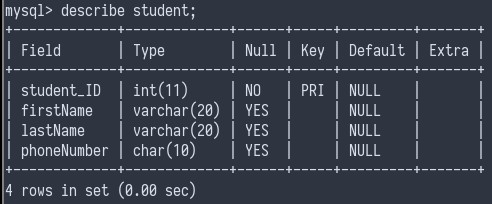
\includegraphics[width=0.8\textwidth]{hw10_5_4}
			\label{fig:hw_10_5_4}
		\end{figure}
	\end{solution}

	\begin{problem}{\#5.5}
		Consider an SQL statement:\\
		\verb|SELECT|\\
		\verb|id, forename, surname|\\
		\verb|FROM|\\
		\verb|authors|\\
		\verb|WHERE|\\
		\verb|forename = 'john' AND surname = 'smith'|
		\begin{enumerate}[label=\alph*]
			\item What is this statement intended to do?
			\item Assume that the forename and surname fields are being gathered
				from user supplied input, and suppose the user responds with:\\
				Forename: jo'hn\\
				Surname: smith\\
				What will be the effect?
			\item Now suppose the user responds with:\\
				Forename: jo';drop table authors--\\
				Surname: smith\\
				What will be the effect?
		\end{enumerate}
	\end{problem}
	\begin{solution}
		\begin{enumerate}[label=\alph*]
			\item The statement is supposed to give a list of the IDs, forenames, and
				surnames of all rows in the authors table where the forename is
				john, and the surname is smith.
			\item The apostrophe in the middle of jo'hn will end the query for the forename.
				Meaning that the user will only search jo in the forenames.
			\item Assuming no sanitation of inputs, the apostrophe will end the forename
				section of the query, the semicolon will end the entire query, and
				the command \verb|drop table authors--| will remove the authors table
				from the database, the double hyphens are to comment our the rest of the
				line after the injection attempt.
		\end{enumerate}
	\end{solution}

	\begin{problem}{\#5.8}
		Assume that A, B, and C grant certain privileges on the employee table to X, who
		in turn grants them to Y, as shown in the following table, with the numerical
		entries indicating the time of granting:
		\begin{center}
			\begin{tabular}{|c|c|c|c|c|c|}
				\hline
				\textbf{UserID} & \textbf{Table} & \textbf{Grantor} & \textbf{READ} & \textbf{INSERT} & \textbf{DELETE}\\
				\hline
				X & Employee & A & 15 & 15 & --\\
				\hline
				X & Employee & B & 20 & -- & 20\\
				\hline
				Y & Employee & X & 25 & 25 & 25\\
				\hline
				X & Employee & C & 30 & -- & 30\\
				\hline
			\end{tabular}
		\end{center}
		At time $t=35$, B issues the command \verb|REVOKE ALL RIGHTS ON employee FROM X|.
		Which access rights, if any, of Y must be revoked, using the conventions defined
		in Section 5.2?
	\end{problem}
	\begin{solution}
		Delete access of user Y should be revoked at $t=35$ because B granted read and delete access
		to X, but A also gave read and insert access to X. After the revoke, X should have read and
		insert from A (at $t=15$ ) and read and delete from C (at $t=30$), X has read, insert, and
		delete. Y gets read, insert and delete from X (at  $t=25$) but X has delete privileges revoked
		at  $t=35$, Y ends with read and insert privileges from X.
	\end{solution}

	\begin{problem}{\#5.9}
		The figure below shows a sequence of grant operations for a specific access
		right on a table. Assume that at $t=70$, B revokes the access right from C, using the
		conventions defined in Section 5.2, show the resulting diagram of access right
		decencies.
		\begin{center}
			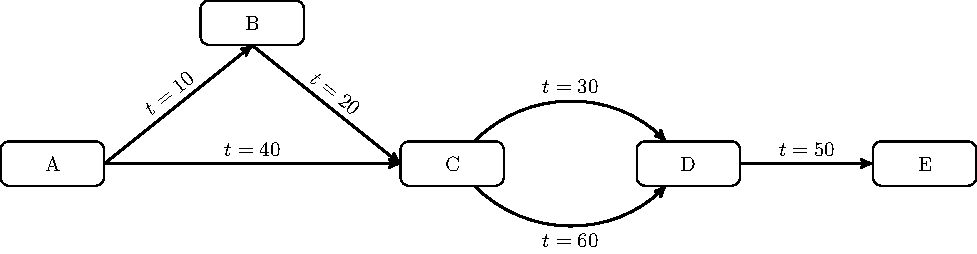
\includegraphics[width=0.9\textwidth]{caspriv.pdf}
		\end{center}
	\end{problem}
	\begin{solution}
		\begin{itemize}
			\item A grants access to B at $t=10$ 
			\item B grants access to C at $t=20$ 
			\item C grants access to D at $t=30$ 
			\item A grants access to C at $t=40$ 
			\item D grants access to E at $t=50$ 
			\item C grants access to D at $t=60$ 
			\item B revokes access from C at $t=70$
		\end{itemize}

		E will be removed from access because E was using privileges given to D from B. When
		B revoked privileges, it cascaded down and removed E. D stays because D was given
		access by C at $t=60$.
		\begin{center}
			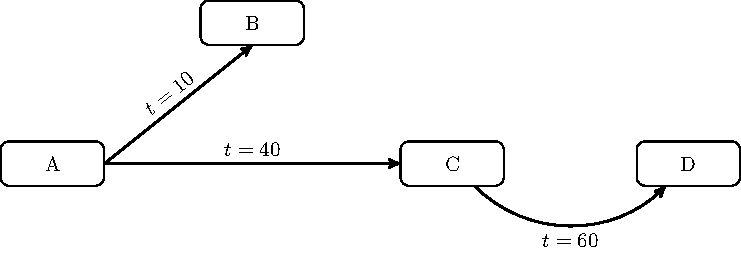
\includegraphics[width=0.8\textwidth]{caspriv1.pdf}
		\end{center}
	\end{solution}

	\begin{problem}{\#5.11}
		Consider the parts department of a plumbing contractor.
		The department maintains an inventory database that includes parts
		information (part number, description, color, size, number in stock,
		etc.) and information on vendors from whom pans are obtained (name,
		address, pending purchase orders, closed purchase orders, etc.). In
		an RBAC system, suppose that roles are defined for accounts payable
		clerk, an installation foreman, and a receiving clerk. For each role,
		indicate which items should be accessible for read-only and read-write
		access.
	\end{problem}
	\begin{solution}
		Accounts Payable Clerk access rights:
		\begin{itemize}
			\item Read
			\item Write
		\end{itemize}
		Installation Foreman access rights:
		\begin{itemize}
			\item Read
		\end{itemize}
		Receiving Clerk access rights:
		\begin{itemize}
			\item Parts -- Read
			\item Parts -- Write
			\item Vendor -- Read
		\end{itemize}
	\end{solution}

	\begin{problem}{\#5.12}
		Imagine that you are the database administrator for a military transportation
		system. You have a table named cargo in your database that contains
		information on the various cargo holds available on each outbound airplane.
		Each row in the table represents a single shipment and lists the contents of
		that shipment and the flight identification number. Only one shipment per hold
		is allowed. The flight identification number may be cross-referenced with other
		tables to determine the origin, destination, flight time, and similar data.
		The cargo table appears as follows:
		\begin{center}
			\begin{tabular}{|c|c|c|c|}
				\hline
				\textbf{Flight ID} & \textbf{Cargo Hold} & \textbf{Contents} & \textbf{Classification}\\
				\hline
				1254 & A & Boots & Unclassified\\
				\hline
				1254 & B & Guns & Unclassified\\
				\hline
				1254 & C & Atomic  Bomb & Top Secret\\
				\hline
				1254 & D & Butter & Unclassified\\
				\hline
			\end{tabular}
		\end{center}
		Suppose that two roles are defined: Role 1 has full access rights to the cargo table.
		Role 2 has access rights only to rows of the table in which the Classification field
		has the value Unclassified. Describe a scenario in which a user assigned to role 2
		uses one or more queries to determine that there is a classified shipment on
		board the aircraft.
	\end{problem}
	\begin{solution}
		If a user with Role 2 tries to insert a item into cargo hold C (because they cannot
		see the classified shipment) they will get an error, in which case the user can deduce
		that there is a classified shipment in cargo hold C.
	\end{solution}
	
	\begin{problem}{\#5.13}
		Users hulkhogan and undertaker do not have the SELECT access right to in Inventory
		table and the Item table. These tables were created by and are owned by user bruno-s.
		Write the SQL commands that would enable bruno-s to grant SELECT access to these tables
		to hulkhogan and undertaker.
	\end{problem}
	\begin{solution}
		The syntax for the grant command is:
		\begin{verbatim}
			GRANT
    			priv_type [(column_list)]
    			  [, priv_type [(column_list)]] ...
    			ON [object_type] priv_level
    			TO user_or_role [, user_or_role] ...
    			[WITH GRANT OPTION]
    			[AS user
    			    [WITH ROLE
    			        DEFAULT
    			      | NONE
    			      | ALL
    			      | ALL EXCEPT role [, role ] ...
    			      | role [, role ] ...
    			    ]
    			]
			}
		\end{verbatim}
		So user bruno-s needs to execute the command:
		\begin{verbatim}
			GRANT select
			ON Inventory
			TO hulkhogan, undertaker
		\end{verbatim}
	\end{solution}
\end{document}
